\documentclass[12pt]{article}
\usepackage{anyfontsize}
\usepackage[a4paper, margin=2cm]{geometry}
\usepackage{polski}
\usepackage[polish]{babel}
\usepackage{tabto}
\usepackage{enumitem}
\usepackage{amsmath}
\usepackage{amssymb}
\usepackage{multirow}
\usepackage{multicol}
\usepackage{setspace}
% \input{verticalPages.tex}

% \usepackage[natbib=true, backend=biber, style=numeric, sorting=none]{biblatex}
% \addbibresource{references.bib}

% \DeclareBibliographyDriver{article}{
%     \printnames{author}
%     \newunit\newblock
%     \printfield{title}
%     \newunit\newblock
%     \usebibmacro{in:}
%     \printfield{journaltitle}
%     \newunit\newblock
%     \printfield{pages}
%     \newunit\newblock
%     \printfield{volume}
%     \newunit
%     \usebibmacro{parenthesis}
%     \printfield{year}
%     \finentry
% }

\usepackage{indentfirst}

\usepackage{subcaption}

\usepackage{tabularx}
\newcolumntype{C}{>{\centering\arraybackslash}X}
\newcolumntype{L}{>{\raggedleft\arraybackslash}X}
\newcolumntype{R}{>{\raggedright\arraybackslash}X}
\newcommand{\centerY}[2]{\multirow{#1}{*}{#2}}

\usepackage{wrapfig}

\usepackage{chngcntr}
\counterwithin{figure}{section}
\counterwithin{table}{section}
\numberwithin{equation}{section}

\usepackage{hyperref}
\hypersetup{
    colorlinks = true,
    urlcolor=blue,
    linkcolor= black,
    citecolor = black
}

\usepackage{graphicx}
\graphicspath{{./Images/}}

\usepackage{csvsimple}
\usepackage{pgfplots}
\usepackage{pgfplotstable}
\pgfplotsset{compat= newest}


\usepackage{titlesec}
\titlelabel{\thetitle.\quad}
% \AddToHook{cmd/section/before}{\clearpage}

\usepackage[european, american currents, americanvoltages, RPvoltages, cute inductor]{circuitikz}
\usepackage{tikz}
\usetikzlibrary{shapes.geometric, decorations.markings, arrows}
\ctikzset{
    logic ports=ieee,
    logic ports/scale=0.7,
}

% \tikzstyle{process} = [rectangle, minimum width=3em, minimum height=2em, text centered, draw=blue, fill=gray!10]
% \tikzstyle{startend} = [ellipse, minimum width=2em, minimum height=1em, text centered, draw=red, fill=gray!10]
% \tikzstyle{startstop} = [rectangle, rounded corners, minimum width=3cm, minimum height=1cm,text centered, draw=black, fill=red!30]
% \tikzstyle{io} = [trapezium, trapezium left angle=70, trapezium right angle=110, minimum width=3cm, minimum height=1cm, text centered, draw=black, fill=blue!30]
% \tikzstyle{process} = [rectangle, minimum width=3cm, minimum height=1cm, text centered, draw=black, fill=orange!30]
% \tikzstyle{decision} = [diamond, minimum width=3cm, minimum height=1cm, text centered, text width = 2.5cm, draw=black, fill=green!30]
% \tikzstyle{arrow} = [thick,->,>=stealth]


\title{
    \vspace*{-1.5cm}
    
\includegraphics[width = 0.25\textwidth]{agh_logo.jpg}\\
    \textbf{Akademia Górniczo-Hutnicza \\im. Stanisława Staszica w Krakowie}\\\vspace{0.5cm}
    Raport z projektu\\\vspace{0.5cm}
    \textbf{Układ do pomiaru natężenia prądu poniżej jednego LSB przetwornika A/C}\\\vspace{0.5cm}
    \small{z przedmiotu}\\\vspace{0.5cm}
    \huge{\textbf{Analogowe układy peryferyjne w systemach cyfrowych}}\\\vspace{0.5cm}
    \small{Elektronika i telekomunikacja - Systemy wbudowane, rok II studiów magisterskich}
}
\author{Piotr Kowol, Michał Nizioł}
\date{\vspace{1cm}\today}

\usepackage{titling}
\renewcommand\maketitlehooka{\null\mbox{}\vfill}
\renewcommand\maketitlehookd{\vfill\null}

\newcommand\inlineeqno{\hfill \stepcounter{equation}\ (\theequation)}
% \newcommand\scheme{\renewcommand{\figurename}{Schemat}}
% \newcommand\plot{\renewcommand{\figurename}{Wykres}}
% \newcommand\photo{\renewcommand{\figurename}{Zdjęcie}}

\begin{document}
    \begin{titlepage}
        \maketitle
        \thispagestyle{empty}
        % \newpage
        % \ 
        % \thispagestyle{empty}
    \end{titlepage}
    
    % \pagenumbering{Roman}
        % \include{shorts.tex}
        \tableofcontents
        % \newpage
        \listoffigures
        \newpage
        % \listoftables
        % \newpage
    % \pagenumbering{gobble}
    \section{Wstęp}
    \subsection{Założenia}
        \begin{itemize}
            \item Pomiar prądu rzędu $10\ nA$,
            \item Wykorzystanie ditheringu szumem Gaussowskim, 
            \item Wykorzystanie mikroprocesora STM32F103C8T6 z 12 bitowym ADC,
            \item Wykorzystanie wzmacniacza pomiarowego INA333.
        \end{itemize}
    \subsection{Schemat Blokowy}
    \begin{figure}[!ht]
        \centering
        \scalebox{1}{\begin{subfigure}{\textwidth}
    \hspace{0cm}
    \begin{tikzpicture}
        \draw
            (0, 0) node[op amp](amp1){}
            (0, -3) node[draw, rectangle, minimum width = 2cm, minimum height = 2cm, label = {[align = center]center:$V_{REF}$}](REF){}
            (3, -3) node[draw, rectangle, minimum width = 2cm, minimum height = 2cm, label = {[align = center]center:Noise \\Gen}]{}
            (5.5, -1) node[adder] (add) {}
            (7.5, -1) node[draw, rectangle, minimum width = 2cm, minimum height = 2cm, label = {[align = center]center:LPF}](LPF){}
            (12, -1) node[draw, rectangle, minimum width = 3cm, minimum height = 5cm, label = {[align = center]center:MCU}](MCU){}
            (12, -6) node[draw, rectangle, minimum width = 2cm, minimum height = 2cm, label = {[align = center]center:USB}](USB){}
            (7, -6) node[draw, rectangle, minimum width = 2cm, minimum height = 2cm, label = {[align = center]center:PSU}](PSU){}
            % (add.135) ++ (-1, 1) -- ++ (0.5, 0) -- (add)
            (add.225) ++ (-1.15, -1) -- ++ (0.5, 0) -- (add) 
            (add) -- ++ (1, 0)

            (amp1) ++ (0.3, -0.3) -- ++ (0, -1.7)
            (amp1.out) -- ++ (3.7, 0) -- (add)
            (amp1.+) -- ++ (-1, 0) to[/tikz/circuitikz/bipoles/length=20pt, R, l=$R_{meas}$] ++ (0, 1)
            (amp1.-) -- ++ (-1, 0) to[short, -o] ++ (0, 1) node[above]{$in-$}
            (amp1.+) ++ (-1, 0) to[short, -o] ++ (0, -1) node[below]{$in+$}
            (LPF) ++ (1, 0) -- ++ (2, 0) ++ (-0.75, 0) node[above]{$ADC_{in}$}
            (USB) ++ (0.5, 1) -- ++ (0, 1.5) ++ (0, -0.75) node[right]{$D-$}
            (USB) ++ (-0.5, 1) -- ++ (0, 1.5) ++ (0, -0.75) node[left]{$D+$}
            (PSU) ++ (1, 0) -- ++ (3, 0) ++ (-1, 0) node[above]{$+5\ V$}
            (PSU) ++ (-1, 0) to[short, -o] ++ (-1, 0) node[above]{$+3.3\ V$}
        ;
            % wzmacniacz pomiarowy, zrodlo ref, generacja szumu, sumator, MCU, USB, PSU, LPF
    \end{tikzpicture}
\end{subfigure}}
        \caption{Schemat blokowy układu do pomiaru natężenia prądu.}
        \label{sch:BD}
    \end{figure}

    \section{Schematy ideowe układu}
    \begin{figure}[!ht]
        \centering
        \scalebox{1}{\begin{subfigure}{\textwidth}
    \hspace{3cm}
    \begin{tikzpicture}
        \draw
            (0, 0) node[op amp, scale = 2](amp){} node[]{INA333}
            (amp) ++ (-1.66, -0.5) -- ++ (-1.22, 0) to[/tikz/circuitikz/bipoles/length=30pt, R, l=$R_G$, a=$10\ \Omega$] ++ (0, 1) -- ++ (1.22, 0)
            (amp.up) to[short, -o] ++ (0, 0.5) node[above]{$3.3\ V$}
            (amp.down) node[ground]{}
            (amp.+) -- ++ (-2.75, 0) to[R, l=$R_{meas}$, a=$100\ \Omega$] ++ (0, 1.96)
            (amp.-) -- ++ (-2.75, 0)
            (amp.+) ++ (-2.75, 0) to[short, *-o] ++ (0, -0.5) node[below]{$In_+$}
            (amp.-) ++ (-2.75, 0) to[short, *-o] ++ (0, 0.5) node[above]{$In_-$}

            (amp) ++ (1, -0.4) to[short, -o] ++ (0, -1) node[below]{$V_{REF}$}
            (amp.out) to[short, -o] ++ (1, 0) node[above]{$V_{out}$}

            (amp.+) ++ (-1, -2) node[below]{$V_{REF}$} to[R, o-*, l=$R_1$, a=$100\ k\Omega$] ++ (0, 2) 
        ;
    \end{tikzpicture}
\end{subfigure}
}
        \caption{Schemat ideowy wzmacniacza pomiarowego.}
        \label{sch:INA333}
    \end{figure}
    \begin{figure}[!ht]
        \centering
        \scalebox{1}{\begin{subfigure}{\textwidth}
    \hspace{0.5cm}
    \begin{tikzpicture}
        \draw
            (0, 0) node[op amp](amp){}
            (amp.up) to[short, -o] ++ (0, 0.5) node[above]{$3.3\ V$}
            (amp.down) node[ground]{}
            (amp.-) -| ++ (-0.5, 1.5) -| ++ (2.98, -2)
            (amp.out) -- ++ (0.1, 0) to[short, *-o] ++ (1, 0) node[above]{$V_{REF}$}
            (amp.out) ++ (0.1, -3) node[ground]{} to[C, l=$C_1$, a=$100\ nF$] ++ (0, 2) -- ++ (0, 1)
            (amp.+) -- ++ (-9, 0) ++ (0, -2) node[ground]{} to[C, l=$C_2$, a=$100\ nF$] ++ (0, 2)
            (amp.+) ++ (-6, -2) node[ground]{} to[C, -*, l=$C_3$, a=$1\ \mu F$] ++ (0, 2)
            (amp.+) ++ (-3, -2) node[ground]{} to[R, -*, l=$R_2$, a=$10\ k\Omega$] ++ (0, 2)
            to[R, -o, l=$R_1$, a=$10\ k\Omega$] ++ (0, 2) node[above]{$3.3\ V$}
        ;
    \end{tikzpicture}
\end{subfigure}}
        \caption{Schemat ideowy źródła napięcia referencyjnego.}
        \label{sch:Vref_gen}
    \end{figure}
    \begin{figure}[!ht]
        \centering
        \scalebox{1}{\begin{subfigure}{\textwidth}
    \hspace{3.5cm}
    \begin{tikzpicture}
        \draw
            (0, 0) node[ground]{} to[zDo, -*, l=$LM336$] ++ (0, 2) coordinate(out)
            to[R, -o, l=$R_1$, a=$820$] ++ (0, 2) node[above]{$3.3\ V$}
            (out) to[C, -o, l=$C_1$, a=$100\ nF$] ++ (3, 0) node[above]{$V_{out}$}
            (out) ++ (3.3, 0) node[circ, scale = 0.6]{}
            (out) ++ (3.5, 0) node[circ, scale = 0.6]{}
            (out) ++ (3.7, 0) node[circ, scale = 0.6]{}
            (out) ++ (5, 0) node[plain mono amp]{$?$}
        ;
    \end{tikzpicture}
\end{subfigure}}
        \caption{Schemat układu generacji szumu białego.}
        \label{sch:Noise_gen}
    \end{figure}
    \begin{figure}[!ht]
        \centering
        \scalebox{1}{    \begin{figure}[H]
        \centering
        \includegraphics[width=1\linewidth]{images/sumator_dc.png}
        \caption{Symulacja dc układu sumującego, napięcia wyjściowego(Vout) od napięcia wejściowego (Vin)}
    \end{figure}}
        \caption{Układ sumacyjny dla dodania sygnału pomiarowego i szumu.}
        \label{sch:sumator}
    \end{figure}
    \begin{figure}[!ht]
        \centering
        \scalebox{1}{\begin{subfigure}{\textwidth}
    \hspace{4cm}
    \begin{tikzpicture}
    \draw
        (0, 0) node[draw, rectangle, minimum width = 3cm, minimum height = 3cm, label = {above:LT1117-3.3}](U1){}
        (U1.west) node[right=1mm] {IN}
        (U1.east) node[left=1mm] {OUT}
        (U1.south) node[above=1mm] {GND}
        (U1.south) node[ground]{}

        (U1.west) -- ++(-2,0) coordinate(IN)
        to[C, l=$C_{1}$, a=$10\ \mu$F] (IN |- U1.south) node[ground] {}
        (IN) to[short, -o] ++ (-1, 0) node[above]{$5V$}

        (U1.east) -- ++(2,0) coordinate(OUT)
        to[C, l=$C_{2}$, a=$100\ \mu$F] (OUT |- U1.south) node[ground] {}
        (OUT) to[short, -o] ++ (1, 0) node[above]{$3.3V$}

        ;
    \end{tikzpicture}
\end{subfigure}}
        \caption{Układ stabilizacji napięcia na 3.3V. }
        \label{sch:psu}
    \end{figure}
    \clearpage
    \section{Symulacje układów}
    \begin{figure}[!ht]
        \centering
        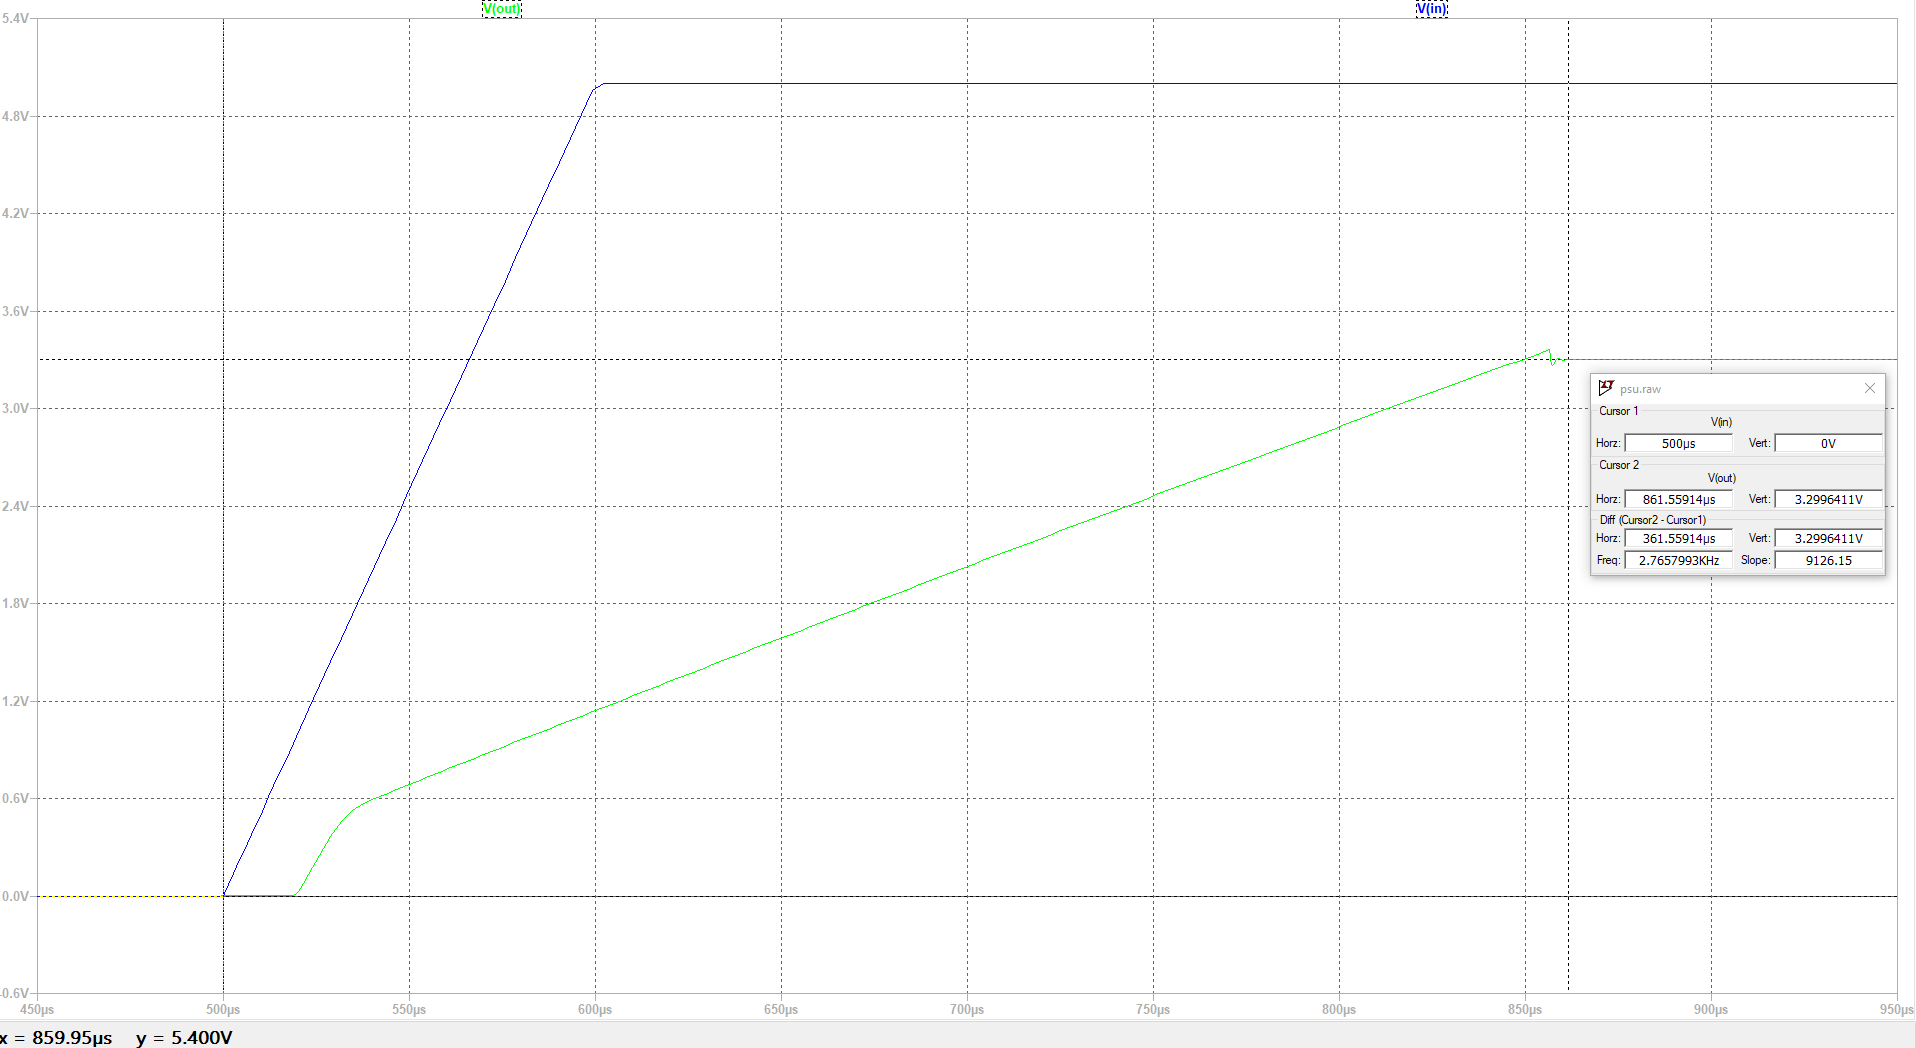
\includegraphics[width=\textwidth]{psu_tran.png}
        \caption{Symulacja tran stabilizatora napięcia LM1117-3.3 napięcia wejściowego ($V_{in}$) i wyjściowego ($V_{out}$).}
        \label{fig:sym_LM1117}
    \end{figure}
    \begin{figure}[!ht]
        \centering
        \includegraphics[width=\textwidth]{sumator_dc.png}
        \caption{Symulacja dc układu sumującego, napięcia wyjściowego ($V_{out}$) od napięcia wejściowego ($V_{in}$).}
        \label{fig:sym_sum}
    \end{figure}
    \begin{figure}[!ht]
        \centering
        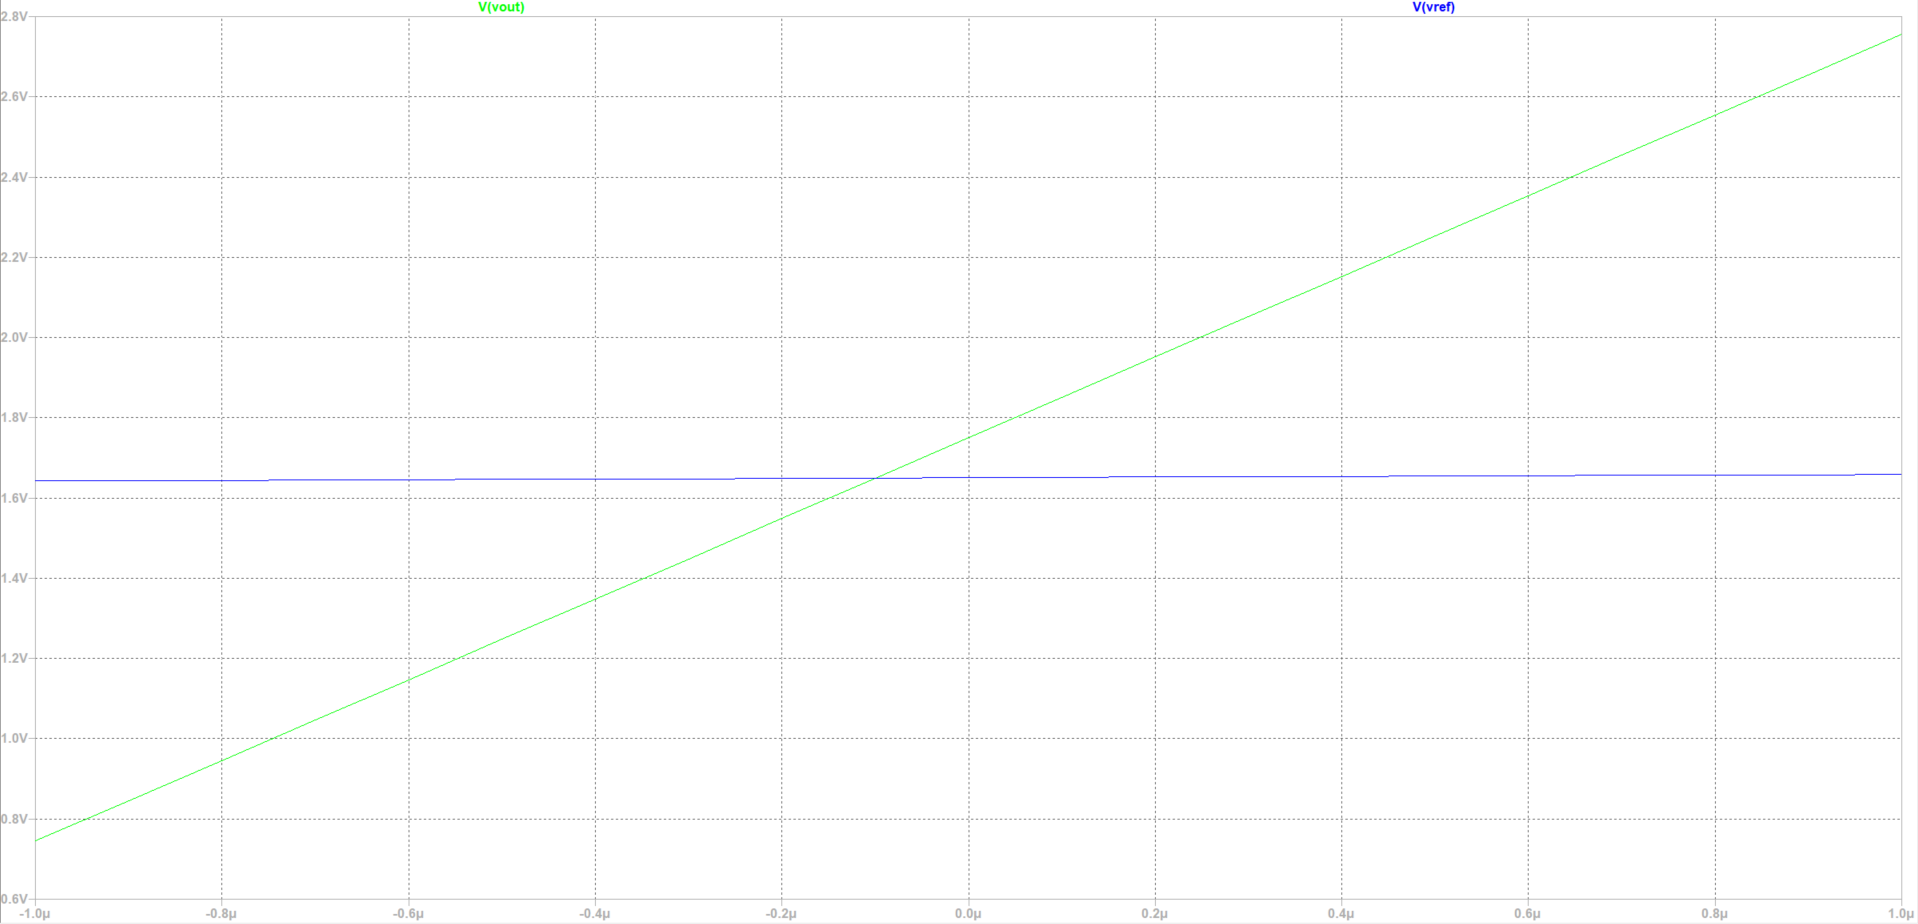
\includegraphics[width=\textwidth]{INA333_1u_range.png}
        \caption{Symulacja parametryczna wzmacniacza pomiarowego w zakresie $\pm 1\ \mu A$.}
        \label{fig:sym_INA_1u}
    \end{figure}
    \begin{figure}[!ht]
        \centering
        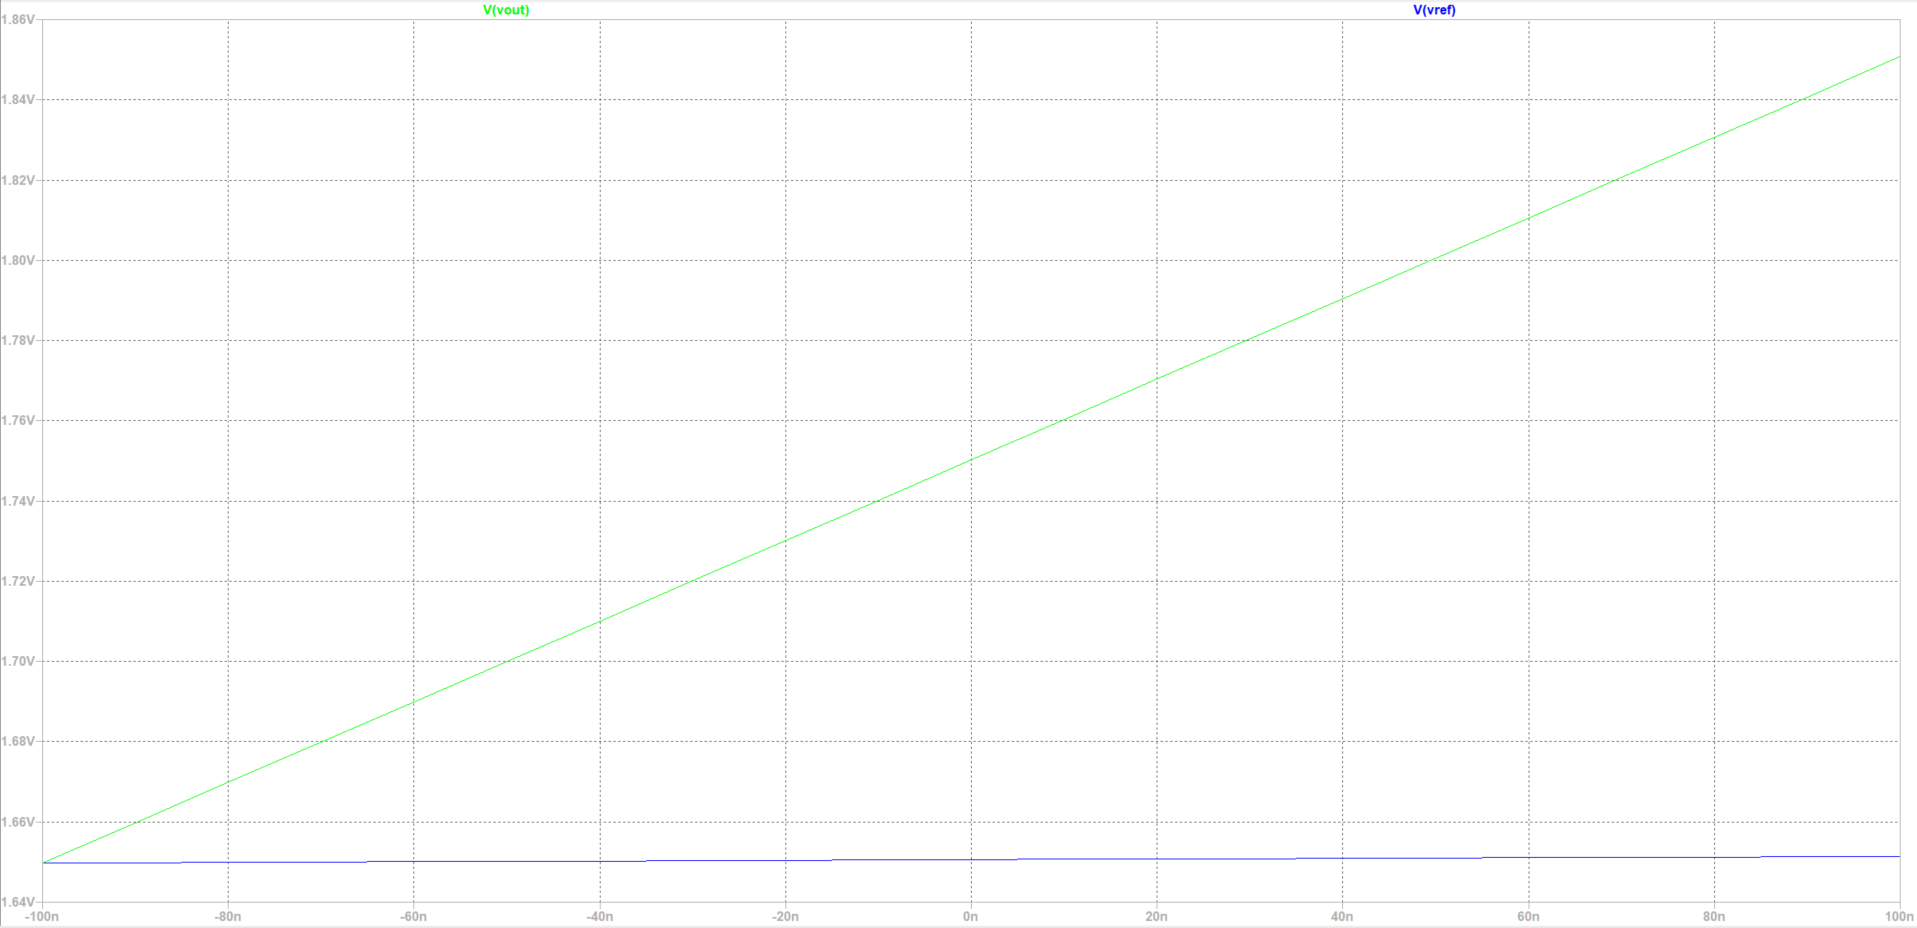
\includegraphics[width=\textwidth]{INA333_100n_range.png}
        \caption{Symulacja parametryczna wzmacniacza pomiarowego w zakresie $\pm 100\ nA$.}
        \label{fig:sym_INA_100n}
    \end{figure}

    % \section{Wstęp}
    \subsection{Założenia}
        \begin{itemize}
            \item Pomiar prądu rzędu $10\ nA$,
            \item Wykorzystanie ditheringu szumem Gaussowskim, 
            \item Wykorzystanie mikroprocesora STM32F103C8T6 z 12 bitowym ADC,
            \item Wykorzystanie wzmacniacza pomiarowego INA333.
        \end{itemize}
    \subsection{Schemat Blokowy}
    \begin{figure}[!ht]
        \centering
        \scalebox{1}{\begin{subfigure}{\textwidth}
    \hspace{0cm}
    \begin{tikzpicture}
        \draw
            (0, 0) node[op amp](amp1){}
            (0, -3) node[draw, rectangle, minimum width = 2cm, minimum height = 2cm, label = {[align = center]center:$V_{REF}$}](REF){}
            (3, -3) node[draw, rectangle, minimum width = 2cm, minimum height = 2cm, label = {[align = center]center:Noise \\Gen}]{}
            (5.5, -1) node[adder] (add) {}
            (7.5, -1) node[draw, rectangle, minimum width = 2cm, minimum height = 2cm, label = {[align = center]center:LPF}](LPF){}
            (12, -1) node[draw, rectangle, minimum width = 3cm, minimum height = 5cm, label = {[align = center]center:MCU}](MCU){}
            (12, -6) node[draw, rectangle, minimum width = 2cm, minimum height = 2cm, label = {[align = center]center:USB}](USB){}
            (7, -6) node[draw, rectangle, minimum width = 2cm, minimum height = 2cm, label = {[align = center]center:PSU}](PSU){}
            % (add.135) ++ (-1, 1) -- ++ (0.5, 0) -- (add)
            (add.225) ++ (-1.15, -1) -- ++ (0.5, 0) -- (add) 
            (add) -- ++ (1, 0)

            (amp1) ++ (0.3, -0.3) -- ++ (0, -1.7)
            (amp1.out) -- ++ (3.7, 0) -- (add)
            (amp1.+) -- ++ (-1, 0) to[/tikz/circuitikz/bipoles/length=20pt, R, l=$R_{meas}$] ++ (0, 1)
            (amp1.-) -- ++ (-1, 0) to[short, -o] ++ (0, 1) node[above]{$in-$}
            (amp1.+) ++ (-1, 0) to[short, -o] ++ (0, -1) node[below]{$in+$}
            (LPF) ++ (1, 0) -- ++ (2, 0) ++ (-0.75, 0) node[above]{$ADC_{in}$}
            (USB) ++ (0.5, 1) -- ++ (0, 1.5) ++ (0, -0.75) node[right]{$D-$}
            (USB) ++ (-0.5, 1) -- ++ (0, 1.5) ++ (0, -0.75) node[left]{$D+$}
            (PSU) ++ (1, 0) -- ++ (3, 0) ++ (-1, 0) node[above]{$+5\ V$}
            (PSU) ++ (-1, 0) to[short, -o] ++ (-1, 0) node[above]{$+3.3\ V$}
        ;
            % wzmacniacz pomiarowy, zrodlo ref, generacja szumu, sumator, MCU, USB, PSU, LPF
    \end{tikzpicture}
\end{subfigure}}
        \caption{Schemat blokowy układu do pomiaru natężenia prądu.}
        \label{sch:BD}
    \end{figure}

    % \input{chapters/zalozenia.tex}
    % \input{chapters/analiza.tex}
    % \input{chapters/opisProjektu.tex}
    % \clearpage
    % \input{chapters/instrukcja.tex}
    % \clearpage
    % \section*{Historia wersji}
    % \begin{table}[!ht]
    %     \centering
    %     \caption{Historia wersji dokumentacji wraz z opisem zmian}
    %     \begin{tabular}{|c|c|c|}\hline
    %         Data wydania & Wersja & Opis \\\hline
    %         15.06.2025 & 1.0.0 & Pierwsza wersja dokumentacji \\\hline
    %     \end{tabular}
    % \end{table}

    % \nocite{*}
    % \bibliographystyle{ieee}
    % \printbibliography

    % \clearpage
    % \input{Chapters/Appendix.tex}
    \vfill
    \begin{flushright}
        Piotr Kowol, Michał Nizioł
    \end{flushright}
\end{document}